\documentclass{article}
\usepackage{tikz, comment}
\usepackage{pifont}
\usepackage{fontspec}
\usetikzlibrary{arrows, decorations.markings, decorations.pathreplacing}
\begin{comment}
:Title: Not defined yet
:Slug: No name yet

Description Here.........
\end{comment}
\begin{document}\centering 

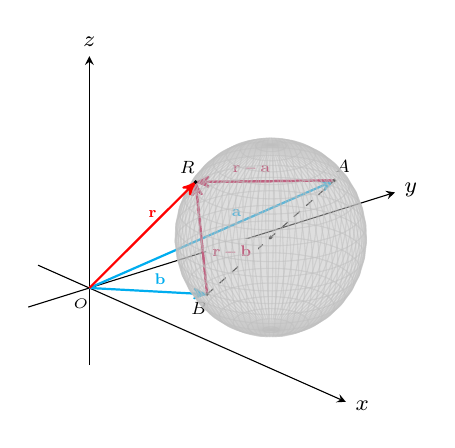
\begin{tikzpicture}[font=\footnotesize]
\pgfplotsset{compat=1.8}

\begin{axis}[axis lines = center, view={50}{30}, ticks=none, scale=1.25,
axis background, xlabel = {$x$}, ylabel ={$y$}, zlabel ={$z$},
xmin =-1,
xmax =5,
ymin =-1,
ymax =5,
zmin =-1, 
zmax =3,
z buffer=sort, data cs=polar, shader=flat,
every axis x label/.style={
    at={(ticklabel* cs:1)},
    anchor= west, yshift =-1.5
},
every axis y label/.style={
    at={(ticklabel* cs:1)},
    anchor= west, yshift =1
},
every axis z label/.style={
    at={(ticklabel* cs:1)},
    anchor= south
}]

\addplot3 [cyan, thick, ->, >=stealth', data cs=cart] coordinates
{ (0,0,0) ({1.75+1.2*cos(30)*sin(45)},{1.5+1.2*sin(30)*sin(45)},{0.8+1.2*cos(45)})}
node[above, midway, pos=0.6, xshift=0, yshift=0, scale=0.7]{${\bf a}$};

\addplot3 [cyan, thick, ->, >=stealth', data cs=cart] coordinates
{ (0,0,0) ({1.75-1.2*cos(30)*sin(45)},{1.5-1.2*sin(30)*sin(45)},{0.8-1.2*cos(45)})}
node[above, midway, pos=0.6, xshift=0, yshift=0, scale=0.7]{${\bf b}$};

\addplot3 [purple, thick, <-, >=stealth', data cs=cart] coordinates
{ ({1.75-1.2*cos(20)*sin(115)},{1.5-1.2*sin(20)*sin(115)},{0.8-1.2*cos(115)}) 
({1.75+1.2*cos(30)*sin(45)},{1.5+1.2*sin(30)*sin(45)},{0.8+1.2*cos(45)}) };

\addplot3 [purple, thick, ->, >=stealth', data cs=cart] coordinates
{ ({1.75-1.2*cos(20)*sin(115)},{1.5-1.2*sin(20)*sin(115)},{0.8-1.2*cos(115)}) 
({1.75-1.2*cos(30)*sin(45)},{1.5-1.2*sin(30)*sin(45)},{0.8-1.2*cos(45)}) };

\addplot3 [dashed, data cs=cart] coordinates
{ ({1.75-1.2*cos(30)*sin(45)},{1.5-1.2*sin(30)*sin(45)},{0.8-1.2*cos(45)}) ({1.75+1.2*cos(30)*sin(45)},{1.5+1.2*sin(30)*sin(45)},{0.8+1.2*cos(45)}) };

\addplot3 [purple, thick, <-, >=stealth', data cs=cart] coordinates
{ ({1.75-1.2*cos(20)*sin(115)},{1.5-1.2*sin(20)*sin(115)},{0.8-1.2*cos(115)}) 
({1.75+1.2*cos(30)*sin(45)},{1.5+1.2*sin(30)*sin(45)},{0.8+1.2*cos(45)}) }
node[black, above, xshift=3, scale=0.8]{$A$}
node[above, midway, pos=0.4, xshift=0, yshift=0, scale=0.7]{${\bf r-a}$};

\addplot3 [opacity=0, thick, ->, >=stealth', data cs=cart] coordinates
{ (0,0,0) ({1.75-1.2*cos(30)*sin(45)},{1.5-1.2*sin(30)*sin(45)},{0.8-1.2*cos(45)})}
node[black, below, xshift=-3, scale=0.8, opacity=1]{$B$};

\addplot3 [purple, thick, ->, >=stealth', data cs=cart] coordinates
{ ({1.75-1.2*cos(20)*sin(115)},{1.5-1.2*sin(20)*sin(115)},{0.8-1.2*cos(115)}) 
({1.75-1.2*cos(30)*sin(45)},{1.5-1.2*sin(30)*sin(45)},{0.8-1.2*cos(45)}) }
node[right, fill=white, midway, pos=0.4, xshift=1, yshift=-1, scale=0.7]{${\bf r-b}$};

\node[label={10:{}},circle,fill,inner sep=0.5pt] at (axis cs:1.75,1.5,0.8) {};

\node[label={10:{}},circle,fill,inner sep=0.5pt] at (axis cs:2.48485, 1.92426, 1.64853) {};
\node[label={10:{}},circle,fill,inner sep=0.5pt] at (axis cs:1.01515, 1.07574, -0.0485281) {};

\addplot3 [opacity=0.3, data cs=cart,surf, lightgray, domain = 0:180, domain y=0:360, samples=40]
      ({1.75+1.2*cos(x)*sin(y)},{1.5+1.2*sin(x)*sin(y)},{0.8+1.2*cos(y)});%the sphere

\addplot3 [red, thick, ->, >=stealth', data cs=cart] coordinates
{ (0,0,0) ({1.75-1.2*cos(20)*sin(115)},{1.5-1.2*sin(20)*sin(115)},{0.8-1.2*cos(115)})}
node[left, midway, pos=0.7, xshift=0, yshift=0, scale=0.7]{${\bf r}$}node[black, above, xshift=-3, scale=0.8]{$R$};

\node[label={10:{}},circle,fill,inner sep=0.5pt] at (axis cs:0.728019, 1.12803, 1.30714) {};

\node[label={-110:{\tiny $O$}}] at (axis cs:0,0.2,0.06) {};

\end{axis}
\end{tikzpicture}  
\end{document}